\section{Average Vehicle Speed}
\label{sec:Results_MeanSpeed}

The mean vehicle speed as a function of \ac{mpr} is reported in Table~\vref{tab:MeanSpeed} and illustrated for three critical demand levels in Figures~\vref{fig:MeanSpeed_2077} through \vref{fig:MeanSpeed_3462}. The data reveal several key trends regarding the performance of the Standard, \ac{eco-glosa}, and \ac{flow-glosa} control strategies under the HBEFA4 and PHEMlight5 emission models.

\subparagraph*{1. Systematic Impact of \ac{mpr} on \ac{eco-glosa}.}
A consistent trend across all traffic volumes is the monotonic decrease in average speed under the \ac{eco-glosa} controller as its \ac{mpr} increases. The effect is mild at the lightest load of $69~\unit{\veh\per\hour}$, where the mean speed drops from $13.34~\unit{\metre\per\second}$ to $13.01~\unit{\metre\per\second}$ (a $2.5\%$ reduction) at $100\%$ \ac{mpr} with the HBEFA4 model. However, the speed reduction becomes catastrophic in congested scenarios. At $2769~\unit{\veh\per\hour}$ with the PHEMlight5 model, the average speed collapses from $11.94~\unit{\metre\per\second}$ to just $2.57~\unit{\metre\per\second}$ at $90\%$ \ac{mpr}, a decline of nearly $79\%$. This consistent, downward trend is clearly illustrated in Figures~\vref{fig:MeanSpeed_HBEFA4_2077} and \vref{fig:MeanSpeed_PHEM_2077}.

\begin{figure}[htb]
  \centering
  \begin{subfigure}[b]{0.49\textwidth}
    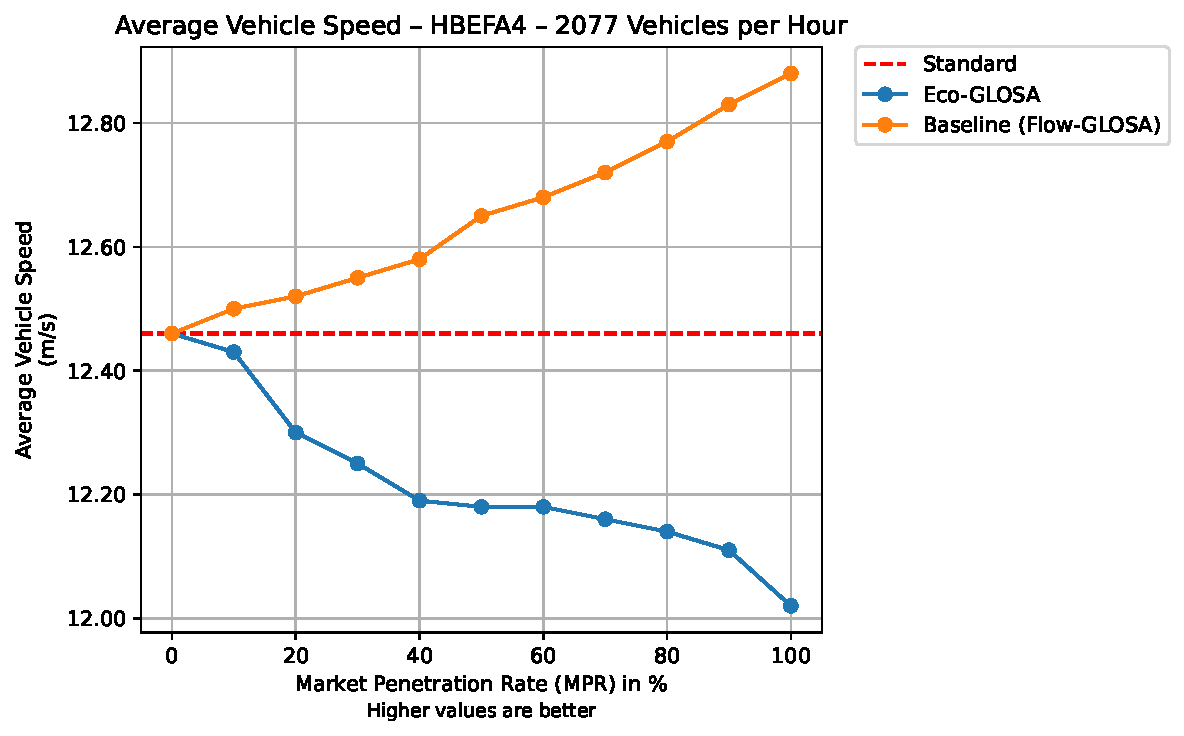
\includegraphics[width=\textwidth]{data/img/AverageVehicleSpeed/AverageVehicleSpeed_HBEFA4_Cars2077.pdf}
    \caption{Mean vehicle speed as a function of \ac{mpr} for the HBEFA4 emission model at a demand level of $2077\,\mathrm{veh/h}$.}
    \label{fig:MeanSpeed_HBEFA4_2077}
  \end{subfigure}\hfill
  \begin{subfigure}[b]{0.49\textwidth}
    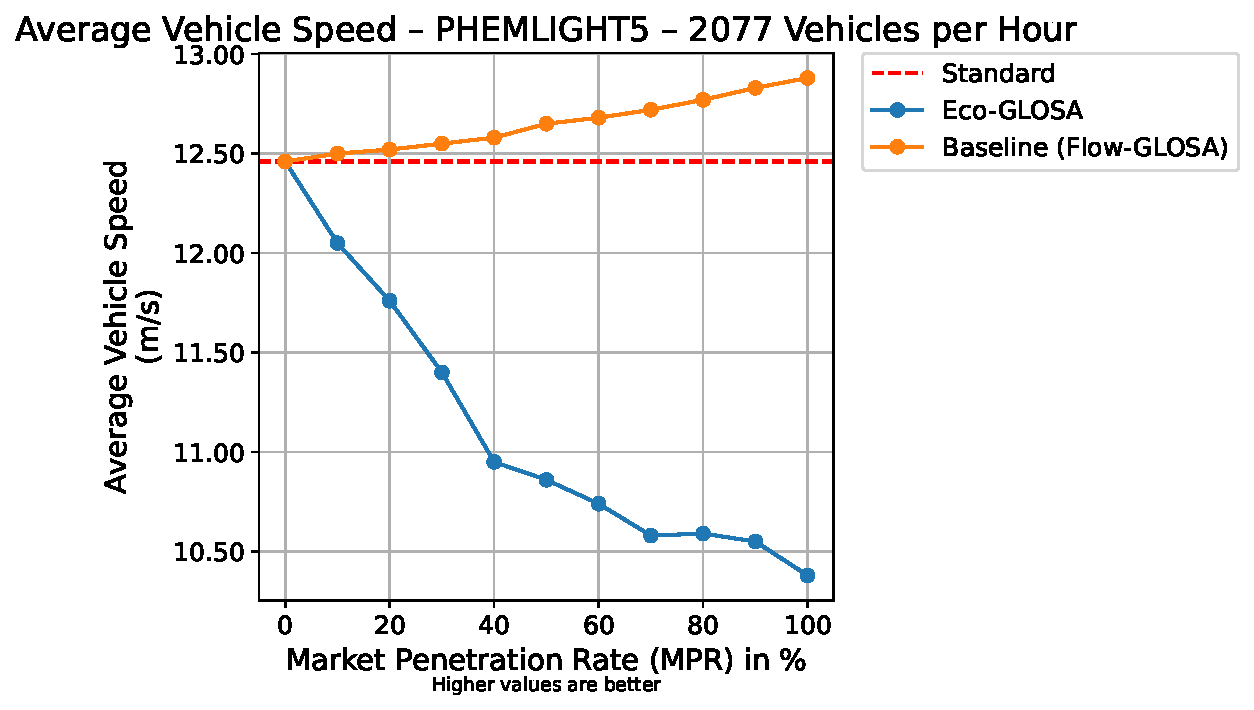
\includegraphics[width=\textwidth]{data/img/AverageVehicleSpeed/AverageVehicleSpeed_PHEMLIGHT5_Cars2077.pdf}
    \caption{Mean vehicle speed as a function of \ac{mpr} for the PHEMlight5 emission model at a demand level of $2077\,\mathrm{veh/h}$.}
    \label{fig:MeanSpeed_PHEM_2077}
  \end{subfigure}
  \caption[Mean vehicle speed vs. \ac{mpr} at $2077~\unit{\veh\per\hour}$]{Mean vehicle speed as a function of \ac{mpr} at a demand of $2077~\unit{\veh\per\hour}$. The plots compare the Standard, \ac{eco-glosa}, and \ac{flow-glosa} controllers under two different emission models.}
\label{fig:MeanSpeed_2077}
\end{figure}

\subparagraph*{2. Flow Stability and Jam Resolution of \ac{flow-glosa}.}
In contrast, the \ac{flow-glosa} algorithm demonstrates remarkable flow stability. It successfully maintains near-Standard speeds for demands up to $2769~\unit{\veh\per\hour}$. Under fully saturated conditions ($3462~\unit{\veh\per\hour}$), it proves capable of dissolving the traffic jam once penetration exceeds approximately $80\%$. The mean speed increases from a gridlocked $3.86~\unit{\metre\per\second}$ to $12.18~\unit{\metre\per\second}$ at $100\%$ \ac{mpr}. This behaviour confirms that a flow-optimised strategy can actively restore free-flow conditions, as shown in Figures~\vref{fig:MeanSpeed_HBEFA4_3462} and \vref{fig:MeanSpeed_PHEM_3462}.

\begin{figure}[htb]
  \centering
  \begin{subfigure}[b]{0.49\textwidth}
    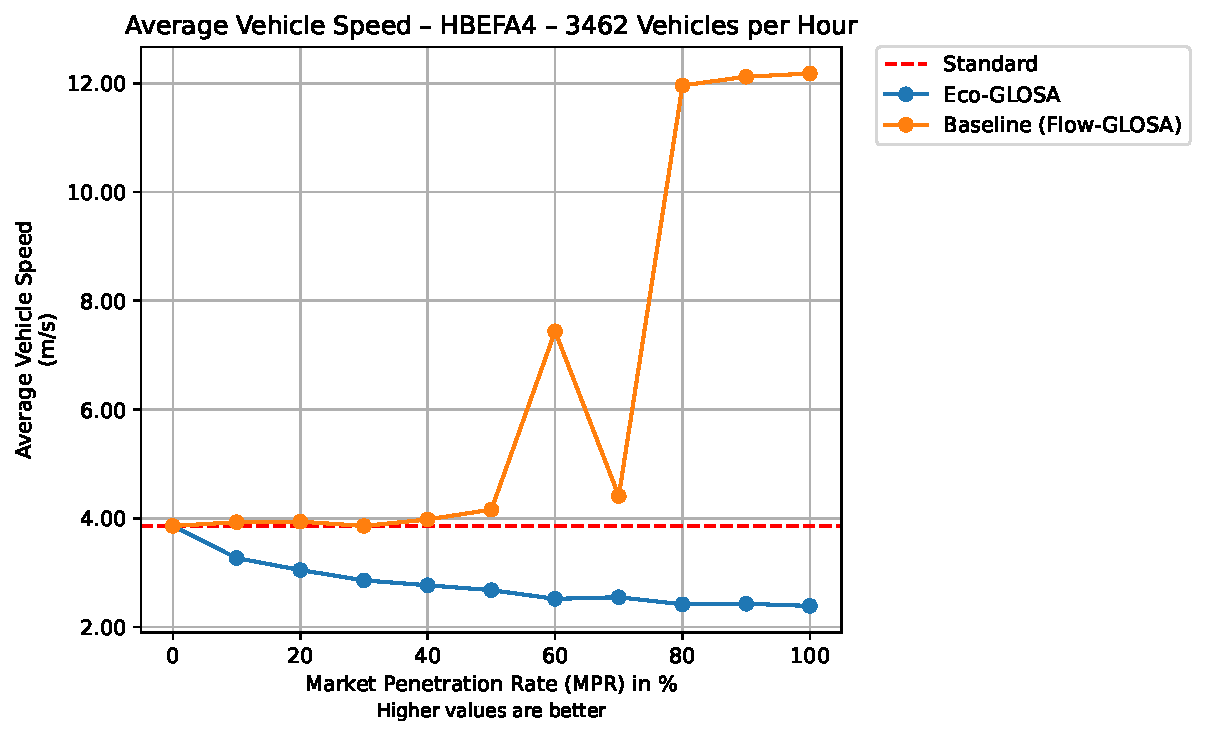
\includegraphics[width=\textwidth]{data/img/AverageVehicleSpeed/AverageVehicleSpeed_HBEFA4_Cars3462.pdf}
    \caption{Mean vehicle speed as a function of \ac{mpr} for the HBEFA4 emission model at $3462\,\mathrm{veh/h}$.}
    \label{fig:MeanSpeed_HBEFA4_3462}
  \end{subfigure}\hfill
  \begin{subfigure}[b]{0.49\textwidth}
    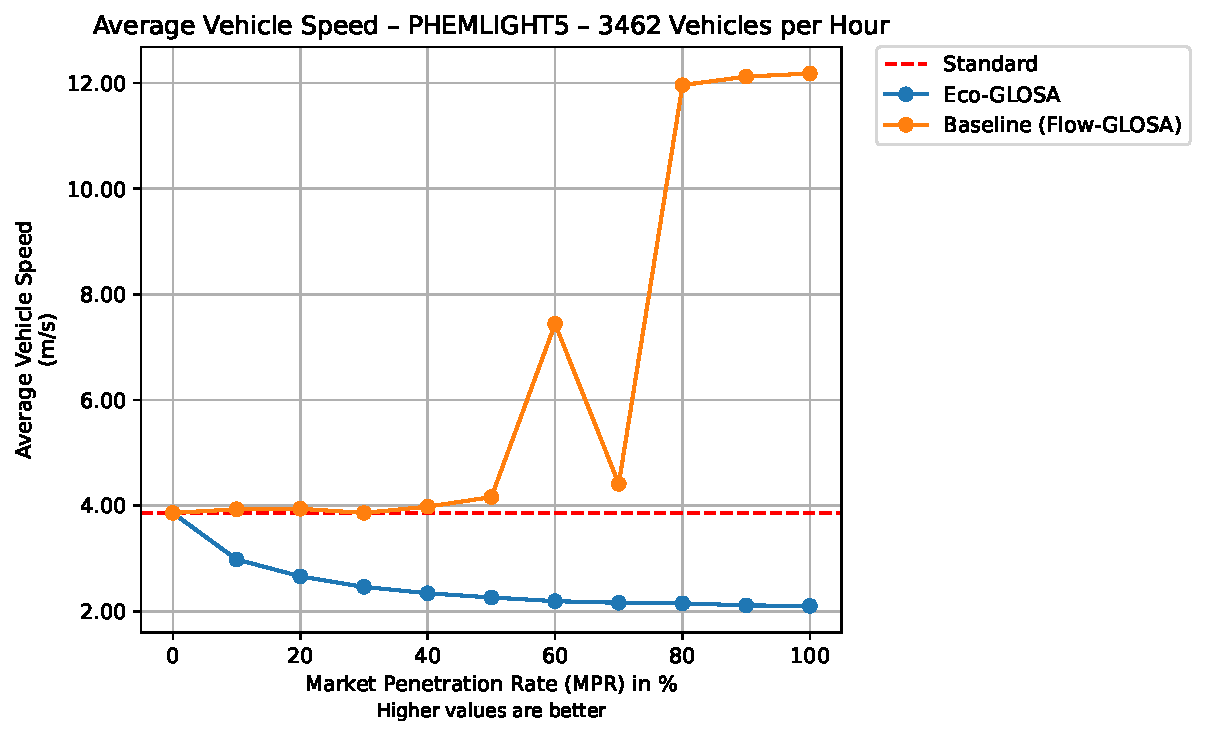
\includegraphics[width=\textwidth]{data/img/AverageVehicleSpeed/AverageVehicleSpeed_PHEMLIGHT5_Cars3462.pdf}
    \caption{Mean vehicle speed as a function of \ac{mpr} for the PHEMlight5 emission model at $3462\,\mathrm{veh/h}$.}
    \label{fig:MeanSpeed_PHEM_3462}
  \end{subfigure}
  \caption[Mean vehicle speed vs. \ac{mpr} at $3462~\unit{\veh\per\hour}$]{Mean vehicle speed as a function of \ac{mpr} in the fully saturated regime of $3462~\unit{\veh\per\hour}$. The results for the Standard, \ac{eco-glosa}, and \ac{flow-glosa} controllers are shown for both the HBEFA4 and PHEMlight5 models.}
\label{fig:MeanSpeed_3462}
\end{figure}

\subparagraph*{3. Emission-Model Sensitivity.}
The choice of emission model significantly influences the simulated speed for the \ac{eco-glosa} controller, particularly in congestion. At $2769~\unit{\veh\per\hour}$ and $60\%$ \ac{mpr}, the HBEFA4 model reports a speed of $3.52~\unit{\metre\per\second}$, whereas the more sensitive PHEMlight5 model shows a lower speed of $2.89~\unit{\metre\per\second}$ (see Figures~\vref{fig:MeanSpeed_HBEFA4_2769} and~\vref{fig:MeanSpeed_PHEM_2769}). This divergence occurs because the PHEMlight5 model more heavily penalises the short bursts of high engine power characteristic of stop-and-go traffic, prompting the eco-controller to adopt even more conservative (slower) speed profiles.

\begin{figure}[htb]
  \centering
  \begin{subfigure}[b]{0.49\textwidth}
    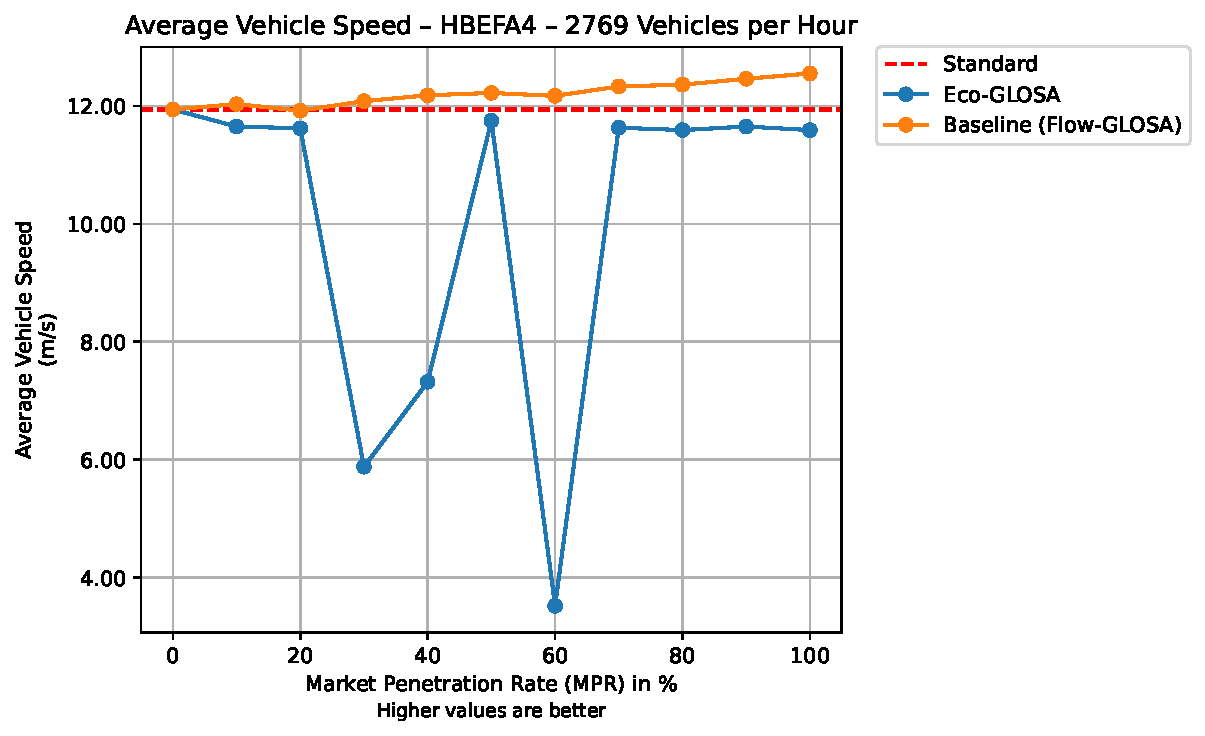
\includegraphics[width=\textwidth]{data/img/AverageVehicleSpeed/AverageVehicleSpeed_HBEFA4_Cars2769.pdf}
    \caption{Mean vehicle speed as a function of \ac{mpr} for the HBEFA4 emission model at $2769\,\mathrm{veh/h}$.}
    \label{fig:MeanSpeed_HBEFA4_2769}
  \end{subfigure}\hfill
  \begin{subfigure}[b]{0.49\textwidth}
    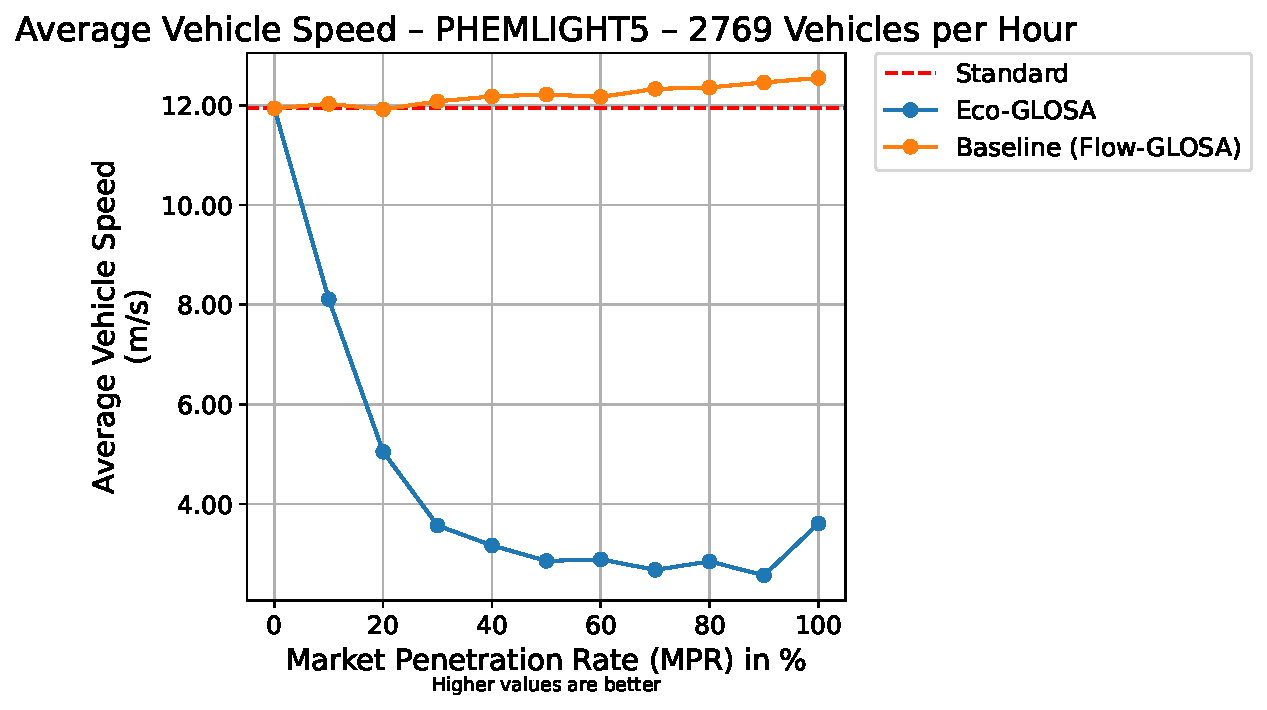
\includegraphics[width=\textwidth]{data/img/AverageVehicleSpeed/AverageVehicleSpeed_PHEMLIGHT5_Cars2769.pdf}
    \caption{Mean vehicle speed as a function of \ac{mpr} for the PHEMlight5 emission model at $2769\,\mathrm{veh/h}$.}
    \label{fig:MeanSpeed_PHEM_2769}
  \end{subfigure}
  \caption[Mean vehicle speed vs. \ac{mpr} at $2769~\unit{\veh\per\hour}$]{Mean vehicle speed versus \ac{mpr} at a congested demand of $2769~\unit{\veh\per\hour}$. The plots illustrate the performance divergence of the Standard, \ac{eco-glosa}, and \ac{flow-glosa} strategies under different emission models.}
\label{fig:MeanSpeed_2769}
\end{figure}

\subparagraph*{4. Jam-Onset Thresholds.}
The data reveal clear breakpoints where traffic flow collapses into a jam, defined as speed falling below $4~\unit{\metre\per\second}$. For a demand of $2769~\unit{\veh\per\hour}$, the PHEMlight5 model shows a jam forming when the \ac{eco-glosa} \ac{mpr} reaches $30\%$. The HBEFA4 model postpones this onset until the \ac{mpr} is higher, at $60\%$. Notably, the average speed under HBEFA4 fluctuates significantly before this point, indicating the system is highly unstable as it approaches its capacity limit. At the highest demand of $3462~\unit{\veh\per\hour}$, both models show the network is already at the jam threshold under Standard conditions, with \ac{eco-glosa} unable to prevent a further collapse in speed at any penetration rate.

\subparagraph*{5. Residual Overshoot at Low Demand.}
In sub-saturated conditions ($69$--$1385~\unit{\veh\per\hour}$), the \ac{eco-glosa} controller occasionally produces average speeds slightly higher than the Standard. The largest overshoot of approximately $0.52~\unit{\metre\per\second}$ occurs at $69~\unit{\veh\per\hour}$ with $10\%$ \ac{mpr}. This effect stems from the algorithm's \enquote{anticipatory glide}, which smooths minor stop-and-go waves present in the baseline traffic, thereby reducing deceleration phases. However, this minor gain is quickly negated as the controller's fuel-saving objective leads to overall lower speeds at higher penetration rates.

\subparagraph*{6. Progressive Speed Gains under \ac{flow-glosa}.}
The \ac{flow-glosa} controller delivers consistent speed improvements as its penetration increases, even in unsaturated conditions. At low demand ($69~\unit{\veh\per\hour}$), the speed increases from $13.34$ to $13.88~\unit{\metre\per\second}$ (a $4.1\%$ gain) at $90\%$ \ac{mpr}. Similarly, at high demand ($2769~\unit{\veh\per\hour}$), it increases from $11.94$ to $12.55~\unit{\metre\per\second}$ (a $5.1\%$ gain) at $100\%$ \ac{mpr}. This progressive uplift underscores the controller's effectiveness at improving throughput across all traffic regimes.

\subparagraph*{Implications.}
A primary distinction arises from the controllers' design philosophies. The advisory logic of \ac{flow-glosa} is purely kinematic, making its performance independent of the chosen emission model. Consequently, its speed curves in Figures~\vref{fig:MeanSpeed_HBEFA4_2077} and \vref{fig:MeanSpeed_PHEM_2077} are identical, providing a stable baseline for comparison. By contrast, the \ac{eco-glosa} controller's behaviour is intrinsically linked to the underlying fuel map. This sensitivity results in markedly different performance outcomes. For example, at a demand of $2077~\unit{\veh\per\hour}$, the transient-sensitive PHEMlight5 model causes speeds to degrade at an \ac{mpr} of just $10\%$, whereas the HBEFA4 model shows speeds remaining stable until a higher penetration is reached.
This divergence becomes most critical in saturated conditions. At a demand of $3462~\unit{\veh\per\hour}$, the \ac{eco-glosa} controller's focus on individual vehicle efficiency is counterproductive and fails to alleviate the gridlock. The \ac{flow-glosa} controller, however, successfully dissolves the queue once the \ac{mpr} exceeds $80\%$. It actively restores free-flow conditions, with average speeds recovering to over $12~\unit{\metre\per\second}$, as shown in Figures~\vref{fig:MeanSpeed_HBEFA4_3462} and \vref{fig:MeanSpeed_PHEM_3462}.
At lighter, sub-saturated volumes ($69$--$1385~\unit{\veh\per\hour}$), the \ac{eco-glosa} controller does offer marginal speed smoothing. This effect can occasionally lead to a slight increase in average speed over the Standard, with a maximum observed overshoot of approximately $0.52~\unit{\metre\per\second}$ at $10\%$ \ac{mpr}. However, this minor gain vanishes as \ac{mpr} increases and the controller's primary objective of saving fuel leads to more conservative speed profiles. Therefore, the deployment strategy for these controllers depends heavily on the operational traffic regime. On lightly loaded arterials, \ac{eco-glosa} may be deployed to fine-tune speed consistency. However, for corridors operating near or above capacity (e.g., $> 2000~\unit{\veh\per\hour}$), the \ac{flow-glosa} algorithm is essential. Its role in these scenarios is not merely to maintain throughput, but to actively prevent network collapse and resolve existing gridlock.

\begin{table}[htb]
  \centering
  \caption[Summary of mean vehicle speed by demand and \ac{mpr}]{A comprehensive summary of mean vehicle speed, in $\unit{\metre\per\second}$, tabulated by traffic demand and \ac{mpr}. The data compares the Standard (no \ac{glosa}), Baseline (\ac{flow-glosa}), and Eco (\ac{eco-glosa}) controller configurations.}
  \label{tab:MeanSpeed}
  \resizebox{\textwidth}{!}{%
  \begin{tabular}{r l l r *{10}{r}}
    \toprule
    Vehicles & Algorithm & Fuel & \textbf{0\% (Std)} & 10\% & 20\% & 30\% & 40\% & 50\% & 60\% & 70\% & 80\% & 90\% & 100\%\\
    \midrule
    69  & \ac{eco-glosa} & HBEFA4 & \textbf{13.34} & 13.86 & 13.45 & 13.71 & 13.51 & 13.46 & 13.71 & 13.72 & 13.05 & 13.81 & 13.01\\
    69  & Baseline (\ac{flow-glosa}) & HBEFA4 & \textbf{13.34} & 13.98 & 13.58 & 13.66 & 13.69 & 13.62 & 13.65 & 13.85 & 13.63 & 13.88 & 13.34\\
    69  & \ac{eco-glosa} & PHEMLIGHT5 & \textbf{13.34} & 13.89 & 13.38 & 13.79 & 13.60 & 12.77 & 13.30 & 13.23 & 12.81 & 13.70 & 12.34\\
    69  & Baseline (\ac{flow-glosa}) & PHEMLIGHT5 & \textbf{13.34} & 13.98 & 13.58 & 13.66 & 13.69 & 13.62 & 13.65 & 13.85 & 13.63 & 13.88 & 13.34\\
    \midrule
    138 & \ac{eco-glosa} & HBEFA4 & \textbf{13.24} & 13.51 & 13.29 & 13.46 & 13.56 & 13.36 & 13.52 & 13.17 & 13.12 & 13.01 & 12.97\\
    138 & Baseline (\ac{flow-glosa}) & HBEFA4 & \textbf{13.24} & 13.52 & 13.37 & 13.41 & 13.65 & 13.47 & 13.57 & 13.52 & 13.41 & 13.39 & 13.23\\
    138 & \ac{eco-glosa} & PHEMLIGHT5 & \textbf{13.24} & 13.38 & 13.40 & 13.36 & 13.64 & 13.15 & 13.39 & 13.03 & 12.99 & 12.70 & 12.50\\
    138 & Baseline (\ac{flow-glosa}) & PHEMLIGHT5 & \textbf{13.24} & 13.52 & 13.37 & 13.41 & 13.65 & 13.47 & 13.57 & 13.52 & 13.41 & 13.39 & 13.23\\
    \midrule
    346 & \ac{eco-glosa} & HBEFA4 & \textbf{13.24} & 13.24 & 13.14 & 13.07 & 13.18 & 13.01 & 13.08 & 13.04 & 12.96 & 12.99 & 12.87\\
    346 & Baseline (\ac{flow-glosa}) & HBEFA4 & \textbf{13.24} & 13.27 & 13.19 & 13.20 & 13.25 & 13.28 & 13.33 & 13.33 & 13.35 & 13.36 & \textbf{13.48}\\
    346 & \ac{eco-glosa} & PHEMLIGHT5 & \textbf{13.24} & 13.20 & 12.83 & 12.71 & 12.80 & 12.77 & 12.56 & 12.59 & 12.52 & 12.64 & 12.50\\
    346 & Baseline (\ac{flow-glosa}) & PHEMLIGHT5 & \textbf{13.24} & 13.27 & 13.19 & 13.20 & 13.25 & 13.28 & 13.33 & 13.33 & 13.35 & 13.36 & \textbf{13.48}\\
    \midrule
    692 & \ac{eco-glosa} & HBEFA4 & \textbf{13.17} & 13.13 & 13.17 & 13.09 & 13.04 & 13.01 & 13.05 & 12.94 & 12.91 & 12.82 & 12.81\\
    692 & Baseline (\ac{flow-glosa}) & HBEFA4 & \textbf{13.17} & 13.23 & 13.25 & 13.20 & 13.27 & 13.22 & 13.36 & 13.25 & 13.31 & 13.39 & 13.33\\
    692 & \ac{eco-glosa} & PHEMLIGHT5 & \textbf{13.17} & 13.08 & 12.95 & 12.71 & 12.68 & 12.52 & 12.49 & 12.38 & 12.24 & 12.11 & 12.10\\
    692 & Baseline (\ac{flow-glosa}) & PHEMLIGHT5 & \textbf{13.17} & 13.23 & 13.25 & 13.20 & 13.27 & 13.22 & 13.36 & 13.25 & 13.31 & 13.39 & 13.33\\
    \midrule
    1385 & \ac{eco-glosa} & HBEFA4 & \textbf{12.84} & 12.75 & 12.75 & 12.74 & 12.69 & 12.62 & 12.59 & 12.55 & 12.51 & 12.49 & 12.41\\
    1385 & Baseline (\ac{flow-glosa}) & HBEFA4 & \textbf{12.84} & 12.82 & 12.81 & 12.82 & 12.93 & 12.90 & 13.00 & 13.00 & 13.08 & 13.03 & 13.07\\
    1385 & \ac{eco-glosa} & PHEMLIGHT5 & \textbf{12.84} & 12.52 & 12.27 & 11.98 & 11.87 & 11.56 & 11.37 & 11.42 & 11.38 & 11.31 & 11.31\\
    1385 & Baseline (\ac{flow-glosa}) & PHEMLIGHT5 & \textbf{12.84} & 12.82 & 12.81 & 12.82 & 12.93 & 12.90 & 13.00 & 13.00 & 13.08 & 13.03 & 13.07\\
    \midrule
    2077 & \ac{eco-glosa} & HBEFA4 & \textbf{12.46} & 12.43 & 12.30 & 12.25 & 12.19 & 12.18 & 12.18 & 12.16 & 12.14 & 12.11 & 12.02\\
    2077 & Baseline (\ac{flow-glosa}) & HBEFA4 & \textbf{12.46} & 12.50 & 12.52 & 12.55 & 12.58 & 12.65 & 12.68 & 12.72 & 12.77 & 12.83 & 12.88\\
    2077 & \ac{eco-glosa} & PHEMLIGHT5 & \textbf{12.46} & 12.05 & 11.76 & 11.40 & 10.95 & 10.86 & 10.74 & 10.58 & 10.59 & 10.55 & 10.38\\
    2077 & Baseline (\ac{flow-glosa}) & PHEMLIGHT5 & \textbf{12.46} & 12.50 & 12.52 & 12.55 & 12.58 & 12.65 & 12.68 & 12.72 & 12.77 & 12.83 & 12.88\\
    \midrule
    2769 & \ac{eco-glosa} & HBEFA4 & \textbf{11.94} & 11.65 & 11.62 & \textbf{5.88} & \textbf{7.32} & 11.75 & \textbf{3.52} & 11.63 & 11.59 & 11.65 & 11.59\\
    2769 & Baseline (\ac{flow-glosa}) & HBEFA4 & \textbf{11.94} & 12.03 & 11.92 & 12.08 & 12.18 & 12.22 & 12.17 & 12.33 & 12.36 & 12.46 & 12.55\\
    \textbf{2769} & \textbf{\ac{eco-glosa}} & \textbf{PHEMLIGHT5} & \textbf{11.94} & \textbf{8.11} & \textbf{5.05} & \textbf{3.57} & \textbf{3.17} & \textbf{2.86} & \textbf{2.89} & \textbf{2.68} & \textbf{2.85} & \textbf{2.57} & \textbf{3.61}\\
    2769 & Baseline (\ac{flow-glosa}) & PHEMLIGHT5 & \textbf{11.94} & 12.03 & 11.92 & 12.08 & 12.18 & 12.22 & 12.17 & 12.33 & 12.36 & 12.46 & 12.55\\
    \midrule
    \textbf{3462} & \textbf{\ac{eco-glosa}} & \textbf{HBEFA4} & \textbf{3.86} & \textbf{3.27} & \textbf{3.05} & \textbf{2.86} & \textbf{2.77} & \textbf{2.68} & \textbf{2.52} & \textbf{2.55} & \textbf{2.42} & \textbf{2.43} & \textbf{2.39}\\
    3462 & Baseline (\ac{flow-glosa}) & HBEFA4 & \textbf{3.86} & 3.93 & 3.94 & 3.86 & 3.98 & 4.16 & \textbf{7.44} & 4.41 & \textbf{11.96} & \textbf{12.12} & \textbf{12.18}\\
    \textbf{3462} & \textbf{\ac{eco-glosa}} & \textbf{PHEMLIGHT5} & \textbf{3.86} & \textbf{2.98} & \textbf{2.66} & \textbf{2.46} & \textbf{2.34} & \textbf{2.26} & \textbf{2.19} & \textbf{2.16} & \textbf{2.15} & \textbf{2.11} & \textbf{2.10}\\
    3462 & Baseline (\ac{flow-glosa}) & PHEMLIGHT5 & \textbf{3.86} & 3.93 & 3.94 & 3.86 & 3.98 & 4.16 & \textbf{7.44} & 4.41 & \textbf{11.96} & \textbf{12.12} & \textbf{12.18}\\
    \bottomrule
  \end{tabular}
  }
\end{table}